\documentclass{article}
\usepackage{textcomp}
\usepackage{graphicx}
\usepackage{amsmath}
\usepackage{siunitx}
\begin{document}


\subsection*{1. 12-bit ADC (Vref = \SI{5}{V})}
\begin{enumerate}
    \item[\bfseries a.] Discrete Values:
        \[ 2^{12} = 4096 \]
    \item[\bfseries b.] Smallest Voltage Step (Resolution):
        \[ \frac{\SI{5}{V}}{2^{12}} = \frac{\SI{5}{V}}{4096} \approx \SI{0.00122}{V} = \SI{1.22}{mV} \]
    \item[\bfseries c.] Output for \SI{3.11}{V} Input:
        \[ \left( \frac{\SI{3.11}{V}}{\SI{5}{V}} \right) \times 4096 = 0.622 \times 4096 \approx 2547.97 \rightarrow \lfloor 2547.97 \rfloor = 2547 \]
\end{enumerate}

\subsection*{2. Square Wave}
\begin{enumerate}
    \item[\bfseries a.] Duty Cycle ($t_{on} = \SI{5}{ms}$, $t_{off} = \SI{10}{ms}$):
        \[ T = t_{on} + t_{off} = \SI{5}{ms} + \SI{10}{ms} = \SI{15}{ms} \]
        \[ \text{Duty Cycle} = \frac{t_{on}}{T} \times 100\% = \frac{\SI{5}{ms}}{\SI{15}{ms}} \times 100\% \approx 33.3\% \]
    \item[\bfseries b.] Increasing $t_{on}$ to \SI{10}{ms} (assuming $T$ changes to \SI{20}{ms}):
        \[ \text{New Duty Cycle} = \frac{\SI{10}{ms}}{\SI{20}{ms}} \times 100\% = 50\% \]
        Effect: LED brightness increases (higher average power).
\end{enumerate}

\subsection*{3. Potentiometer LED Demo}

\begin{center}
\begin{minipage}[t]{0.45\textwidth}
    \includegraphics[width=\textwidth]{potent/a1.png}
\end{minipage}%
\hfill
\begin{minipage}[t]{0.45\textwidth}
    \includegraphics[width=\textwidth]{potent/a2.png}
\end{minipage}

    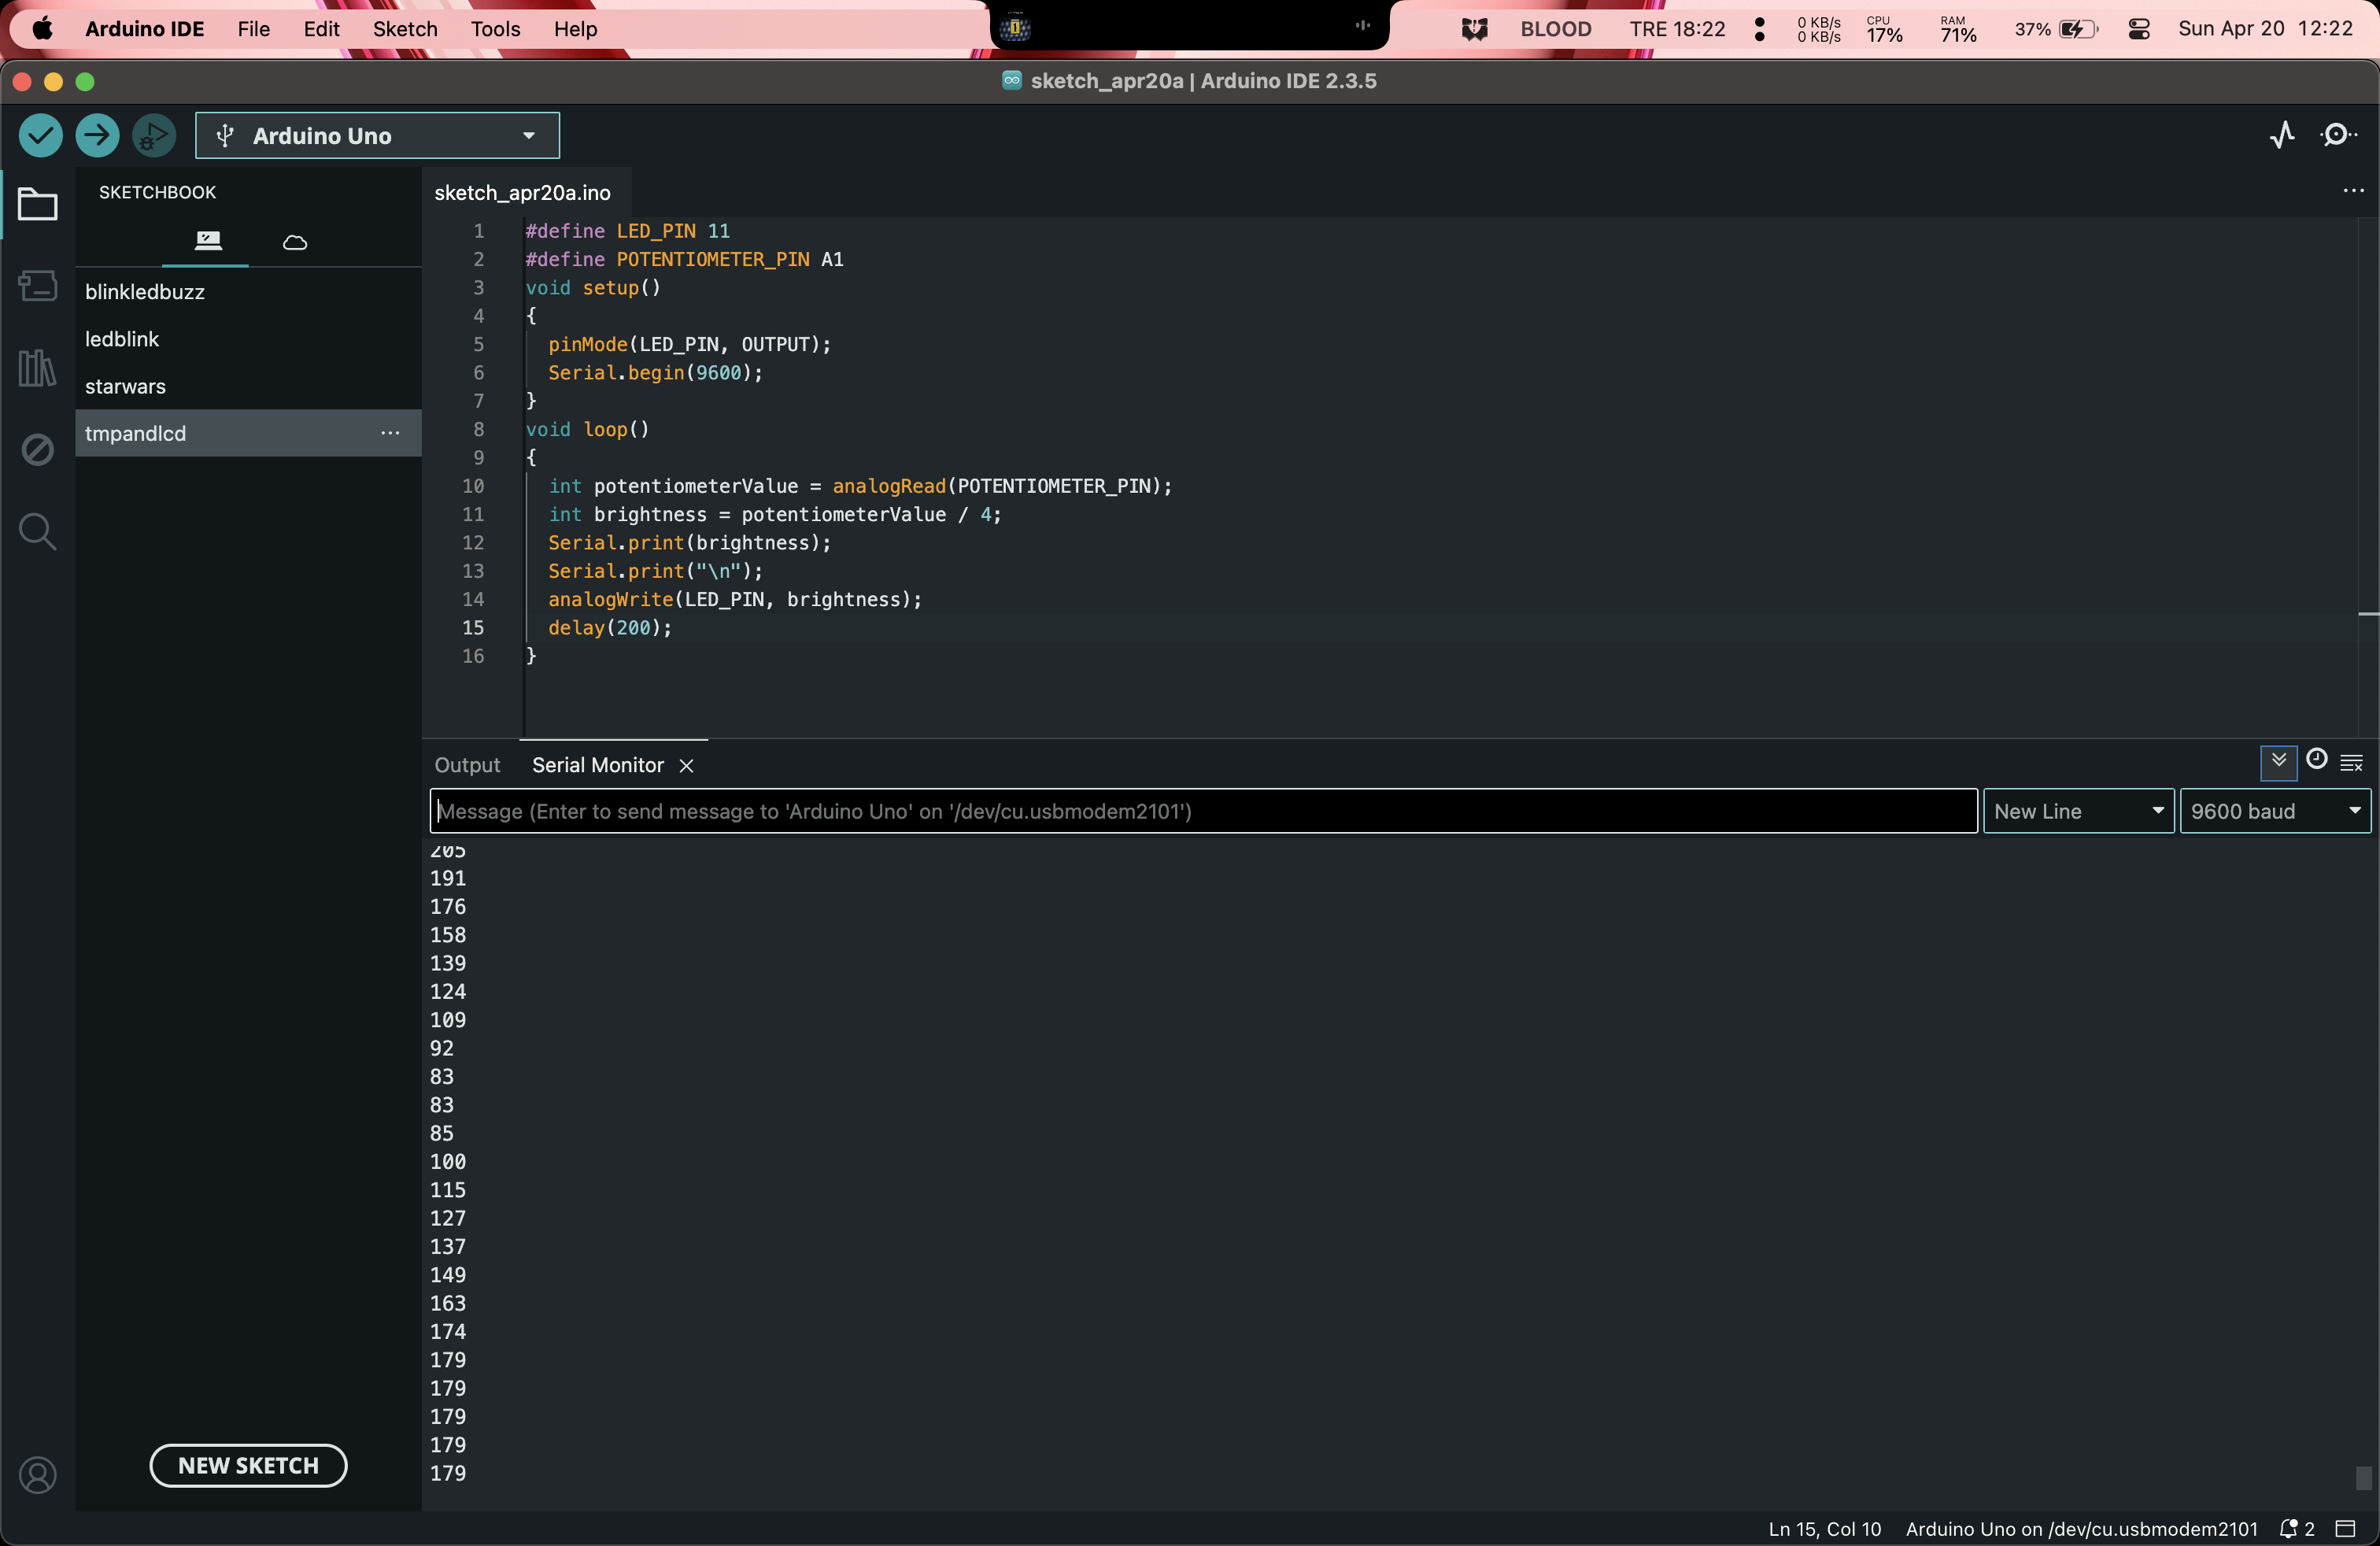
\includegraphics[width=\textwidth]{potent/a4.png}
\end{center}

\subsection*{4. TMP36 Reading}

$$V_{temp}=  V \times (ADC_{in} / 1023)$$
$$V_{temp} = 5 (205 / 1023) = 1,0019550342 $$
\[
  t_{C} = 100 * (V_{temp} - 0.5)
\]

\[
  t_{C} = 100 * (1.0019550342 - 0.5) = 50,2 \, C 
\]


\subsection*{5. Thermistor Circuit}

    \[ V_{A0} = \frac{\text{ADC Reading}}{\text{Total Levels}} \times V_{ref} = \frac{615}{1024} \times \SI{5}{V} \approx \SI{3.003}{V} \]
    \[ V_{A0} = V_{supply} \times \frac{R}{R_T + R} \]
    \[ \SI{3.003}{V} = \SI{5}{V} \times \frac{\SI{10}{k\ohm}}{R_T + \SI{10}{k\ohm}} \]
        \[ R_T = \left( \frac{V_{supply}}{V_{A0}} - 1 \right) R \]
        \[ R_T = \left( \frac{\SI{5}{V}}{\SI{3.003}{V}} - 1 \right) \times \SI{10}{k\ohm} \]
        \[ R_T \approx (1.665 - 1) \times \SI{10}{k\ohm} \approx 0.665 \times \SI{10}{k\ohm} \]
        \[ R_T \approx \SI{6.65}{k\ohm} \]

\[ \text{Temperature} \uparrow \implies R_T \downarrow \]
$R_T$ will \textbf{decrease}.



\end{document}
